%!TEX program = xelatex
\documentclass[11pt,numbers=noenddot]{scrartcl}
\usepackage[ngerman]{babel}
\usepackage[a4paper,lmargin={2.5cm},rmargin={3.5cm}, tmargin={2.5cm},bmargin = {2.5cm}]{geometry}
\usepackage{amsmath}
\usepackage{mathabx}
\usepackage{mathtools}
\usepackage{stmaryrd}
\usepackage{enumitem}
\usepackage{graphicx}

\usepackage{relsize}
% \linespread{1.2}
\usepackage{setspace}
\onehalfspacing
% \usepackage[square]{natbib}
\usepackage{jurabib}
% \usepackage {algorithm2e}

% Package, das die Benutzung von Old Standard erlaubt
\usepackage{fontspec}

\setmainfont{OldStandard-Regular.otf}[
Path = /usr/local/texlive/texmf-local/opentype/,
BoldFont = OldStandard-Bold.otf,
ItalicFont = OldStandard-Italic.otf]

\bibliographystyle{jurabib}
\renewcommand*{\bibbtsep}{In: }
\renewcommand*{\bibjtsep}{In: }
\jurabibsetup{
  authorformat=and
}

% \makeatletter
% % \renewcommand{\l@section}{\@dottedtocline{1}{1.5em}{2.6em}}
% \renewcommand{\l@subsection}{\@dottedtocline{2}{4.0em}{3.6em}}
% \renewcommand{\l@subsubsection}{\@dottedtocline{3}{7.4em}{4.5em}}
% \makeatother

% \addtokomafont{disposition}{\normalfont}
\addtokomafont{sectionentry}{\normalfont\bfseries}


\setkomafont{subject}{\normalfont\small}
\addtokomafont{title}{\normalfont\bfseries}
\addtokomafont{section}{\normalfont\centering\bfseries}
\addtokomafont{subsection}{\normalfont\centering\bfseries}
\addtokomafont{subsubsection}{\normalfont\centering\bfseries}

\addtokomafont{publishers}{\normalfont\small}
\addtokomafont{date}{\normalfont\small}
\addtokomafont{author}{\normalfont\small}
\addtokomafont{descriptionlabel}{\normalfont\bfseries}

% \renewcommand{\thesection}{\Roman{section}} 
% \renewcommand{\thesubsection}{\thesection.\Roman{subsection}}


\subject{  Universität zu Köln \\
  Sprachliche Informationsverarbeitung \\
  Hauptseminar: Angewandte linguistische Datenverarbeitung \\
  Prof. Dr. Jürgen Rolshoven \\
  Hausarbeit
  }
\title{Semantische Spezifität \\im Word Space Model}
\author{Von C. Friedrich}
\date{(Vorgelegt am \today)}


\usepackage{amsthm}
\newtheorem*{defi}{Definition}


\begin{document}
\begin{titlepage}
\maketitle

\abstract{Ladida, ladidu}


\thispagestyle{empty}
\end{titlepage}



\tableofcontents
\newpage

\section{Einleitung}

Weeds et al. (2004) proposed a notion of distributional generality, observing that more general words tend to occur in a larger variety of contexts than more specific words. For example, we would expect to be able to replace any occurrence of cat with animal and so all of the contexts of cat must be plausible
contexts for animal. However, not all of the contexts of animal would be plausible for cat, e.g., “the monstrous animal barked at the intruder”.

\subsection*{Semantische Spezifität}

Was ist die Challenge des Experiments?

\citet[11]{sparckjones1972} Beschreibt die Spezifität eines Begriffes so:
\begin{quote}
  Specificity ... is a semantic property of index terms: a term is more or less specific as its meaning is more or less detailed and precise.
\end{quote}

\subsection*{Semantische Spezifität und Anglizismen}

\section{Ein Maß für die semantische Spezifität}

\subsection{Textgrundlage}

Welche Korpora werden verwendet?

Wie sieht das Präprozessieren aus?

Keine Bigramme.

Frequency Threshold.

\subsection{Score \#1: Document Frequency}
Bereits \citet{sparckjones1972} schlug ein statistisches Maß für die semantische Spezifität eines Wortes vor. Es ist die simple Frequenz, mit der ein Wort im Korpus auftaucht, das ein Indiz für die Spezifität darstellen soll. \citet{Caraballo99determiningthe} konnten die \emph{document frequency} als Eigenschaft von Worten dazu nutzen, für beliebige Wortpaare festzustellen, welches Wort  spezifischer oder genereller ist. Überprüft wurde das mit Beispielwortpaaren, die in einer Hyperonym- bzw. Hyponymrelation zueinander stehen: Das Wort \emph{Getränk} ist ein Oberbegriff zum Wort \emph{Cola}. Für diese Art von Relation gilt: Wenn ein Wort ein Oberbegriff eines anderen ist, so ist der Unterbegriff semantisch spezifischer als der Oberbegriff. Die klar unterschiedene Spezifität ist also eine notwendige Bedingung für die Hyperonym- bzw. Hyponymrelation. Das macht solche Wortpaare zu natürlichen Kandidaten, um Maße für semantische Spezifität zu testen.

Insoweit es die Textgrundlage hergibt, also in Dokumenten geordnet ist, verwende ich die \emph{document frequency} als erste Annäherung an ein brauchbares Maß für die semantische Spezifität. Die Berechnung ist simpel und performant. Entscheidend wird die Frage sein, ob es den komplexeren Modellen gelingt, eine höhere Erfolgsrate zu erzielen. Daher verwende ich die \emph{document frequency} als Benchmark für die anderen Modelle.

Weil das spätere Ziel ist, Worte in unterschiedlichen Korpora miteinander zu vergleichen, muss die \emph{document frequency} noch normiert werden, wodurch das Maß etwas unabhängiger vom verwendeten Korpus wird.

\begin{defi}
Sei $N$ die Gesamtzahl aller untersuchen Dokumente und $df_i$ die Anzahl der Dokumente, in denen das Fokuswort $w_i$ auftritt. Dann ist die \textbf{normierte document frequency} $dfn_i$
\begin{equation}
    dfn_i = \frac{df_i}{N}
\end{equation}
\end{defi}

Hat von zwei Wörtern, die wir miteinander vergleichen wollen das erste eine kleinere $dfn$ als das zweite, ist das nach \citet{Caraballo99determiningthe} eine gute Heuristik, auch eine höhere semantische Spezifität anzunehmen.

\subsection{Das Word Space Model}
Grundlage dieser Arbeit ist das \emph{Word Space Model} (WSM) oder auch Termvektormodell, das unter anderem sehr ausführlich in \citet{sahlgren2006word} beschrieben wird. Das WSM erhält seine Relevanz in der Computerlinguistik hauptsächlich durch eine zentrale Überlegung:
\begin{quote}
    \textbf{The distributional hypothesis:} \emph{words with similar distributional properties have similar meanings.}
\end{quote}
Die Formulierung hier stammt aus \citet[S. 21]{sahlgren2006word}. Die Idee ist naheliegend: Dem abstrakten Konzept der Bedeutungsähnlichkeit wird durch simple räumliche Nähe repräsentiert. Die statistischen Eigenschaften eines Wortes scheinen nach der Hypothese also auf nicht näher bestimmte mit dem semantischen Inhalt eines Wortes zu korrellieren. Diese Korrelation ist jedoch nicht absolut, sondern steht in Relation zu den Eigenschaften eines anderen Wortes. Das WSM stellt also kein Modell für die absolute Bedeutung eines Wortes dar, man kann jedoch Aussagen über die Bedeutungsähnlichkeit verschiedener Worte treffen. \footnote{Je nach Bedeutungstheorie ist das mehr oder minder plausibel. Versteht man Bedeutung primär als Referenz (insbesondere extralinguistisch), so kann diese Analogie nicht viel leisten. Ist vielmehr der Gebrauch des Wortes in der Sprache gefragt, entspricht die Analogie je nach Wahl des konkreten Modells zum Teil sehr deutlich dem Begriff der Bedeutung.}

Zu den statistischen Eigenschaften zählen dabei Phänomene wie die Häufigkeit eines Wortes, die Beziehungen zu anderen Worten in der unmittelbaren Umgebung des Wortes, die Beziehung zu anderen Worten im selben Dokument usw. Das WSM stellt dabei diese Eigenschaften durch Zahlenwerte von verschiedenen Features dar. Ein solches Feature wäre beispielsweise die Häufigkeit des Auftretens eines bestimmten Wortes in direkter Nachbarschaft zum Fokuswort. Die Auswahl dieser Featuremenge legt dabei in sehr relevantem Maße die Aussagen fest, die sich mit Hilfe des WSM treffen lassen. Listet man alle Features eines Fokuswortes auf, so erhält man den Featurevektor des Wortes. Dieser Vektor repräsentiert damit die statistischen Eigenschaften des Fokuswortes im Kontext des Modells, das man ausgewählt hat. Die Ähnlichkeit der Featurevektoren lässt dann Rückschlüsse auf die Bedeutungsähnlichkeit der Worte zu, so die Hypothese.

Um die Ähnlichkeit numerisch bestimmen zu können, braucht es für einen solchen Vektorraum eine Methode, die Distanz zwischen den einzelnen Featurevektoren zu bestimmen. Welche davon sinnvoll eingesetzt werden können, wird in den nächsten Abschnitten beschrieben.

\subsection{Satzkookkurrenzen vs. Fensterkookkurrenzen}

Zunächst müssen die Features, welche die Vektoren ausmachen, festgelegt werden. Ein naheliegender Kandidat sind hier diejenigen Wörter, die mit dem Fokuswort in einer bestimmten Art und Weise gemeinsam auftreten, also kookkurrieren. Über einen gesamten Korpus legen diese Wörter den Kontext des Fokuswortes fest. Nun gibt es mehrere Möglichkeiten, diesen Kontext festzulegen. In dieser Arbeit habe ich die folgenden beiden Ansätze gewählt:

\textbf{Satzkookkurrenzen} sind diejenigen Wörter, mit denen das Fokuswort gemeinsam in einem Satz auftritt. Gezählt werden dabei für zwei Wörter vorranging die Anzahl der Sätze, in denen die Wörter gemeinsam auftreten. Den Satzkontext des Fokuswortes bilden dann die Menge aller Wörter, die mit dem Fokuswort mindestens einmal gemeinsam in einem Satz auftreten.

\textbf{Fensterkookkurrenzen} sind diejenigen Wörter, mit denen das Fokuswort innerhalb eines Fensters von festgelegter Größe gemeinsam auftritt. In Abgrenzung zur Satzkookkurrenz habe ich hier kein symmetrisches Fenster untersucht, sondern nur die nachfolgenden Wörter betrachtet, das rechte, gerichtete Kontextfenster. Die Auswahl der Größe des Fensters ist ebenfalls relevant und führt zu signifikanten Unterschieden.

Der Featurevektor des Fokusworts besteht also aus der Kookkurrenz mit allen anderen Worten des Korpus.

\textbf{Beispiel.} Der Beispieltext
\begin{quote}
    The optional plotz says to frobnicate the bizbaz first. Return a foobang.
\end{quote}
soll analysiert werden mit \emph{plotz} als Fokuswort\footnote{Stopwords wurden bereits entfernt.}:

\begin{table}[h]
    \begin{center}
        \begin{tabular}{ l | *{12}{c}}
                 & optional & plotz & says & frobnicate & bizbaz & first & Return & foobang \\ \hline
            plotz & $k_{1}$ & $k_{2}$ & $k_{3}$ & $k_{4}$ & $k_{5}$ & $k_{6}$ & $k_{7}$ & $k_{8}$ \\ \\
        \end{tabular}
    \end{center}
\end{table}

Die Werte $k_1$ bis $k_8$ sind die Ausprägungen der Relation zwischen den jeweiligen Wörtern. Die Ausprägung hängt davon ab, (i) ob Satzkookkurrenz oder Fensterkookkurrenz verwendet wird und (ii) welches Maß zur Berechnung der Kookkurrenz verwendet wird. Die verschiedenen Maße, die ich verwende, werden in Abschnitt \ref{coocmeasures} vorgestellt.

Paradigmatischer vs. Syntagmatischer Kontext

\subsection{Score \#2: Anzahl der Kookkurenzen}

Ausgehend vom vorherigen Abschnitt lässt sich eine Wort-Wort-Kookkurrenzmatrix erstellen. Diese Matrix enthält alle Featurevektoren jedes einzelnen Wortes des Korpus als Reihe. Die Matrix ist dabei zwingend quadratisch, aber nicht unbedingt symmetrisch, eben im Falle der Fensterkookkurrenzen.

Eine grundlegende These dieser Arbeit ist, das der Kontext eines Wortes als Indiz für seine semantische Spezifität herangezogen werden kann. Nicht nur die reine Häufigkeit eines Wortes ist entscheidend, sondern auch, mit wie vielen verschiedenen Worten das Fokuswort in Kookkurrenz steht. Beispiel: Ein allgemeines Wort kommt etwas seltener vor als ein Spezielleres, der Kontext des spezielleren Wortes ist jedoch beschränkter als der des Allgemeineren, das mit vielen verschiedenen Worten kookkurriert. In so einem Fall würde die \emph{document frequency} fälschlicherweise das allgemeinere Wort als spezieller auszeichnen.

Die Idee dieses Maßes ist es daher, einfach zu zählen, mit wie viele von Null verschiedene Einträge der Featurevektor des Fokuswortes hat, mit anderen Worten, mit wie vielen verschiedenen Worten das Fokuswort in Kookkurrenz steht.

\begin{defi}
Sei $N$ die Gesamtzahl aller (unique) Worte im Korpus und $n_i$ die Anzahl aller (unique) Worte, mit denen das Wort $w_i$ in Kookkurrenz steht, d.h. an dessen Eintrag der Featurevektor von $w_i$ einen von Null verschiedenen Wert aufweist. Dann ist der \textbf{Non-Zero Dimension Score} $nzds_i$
\begin{equation}
    nzds_i = \frac{n_i}{N}
\end{equation}
\end{defi}

Meine These: Ein kleiner $nzds$-Wert eines Wortes spricht für eine höhere semantische Spezifität, ein größerer Wert dafür, dass das Wort eher genereller ist.

\subsection{Maße für die Kookkurrenzen} \label{coocmeasures}

Zusätzlich zur Auswahl der Art der Kookkurrenz muss noch ein Maß zur Bestimmung der Kookkurrenz gewählt werden. In dieser Arbeit habe ich dafür vier verschiedene Maße herangezogen. Ich gebe hier die Maße für den Fall der Fensterkookkurenzen an. Für die Satzkookkurrenzen ergeben sich leicht andere Maße, auch weil die resultierende Matrix symmetrisch ist. Bei direktionalen Kontextfenstern gilt das nicht notwendigerweise (und praktisch fast nie). Daher ist bei jedem Maß zu beachten: score$_{ij}$ ist nicht zwingend gleich score$_{ji}$.

\subsubsection{Binäre Kookkurrenz}

Die binäre Kookkurrenz zeigt an, ob ein Wort mit einem anderen Wort im gesamten Kontext mindestens mit einer bestimmten Frequenz in Kookkurrenz steht.

\begin{defi}
Sei $K_{ij}$ die Menge aller Kontextfenster für Wort $w_i$, in denen das Wort $w_j$ auftritt, und $m$ die Mindestanzahl an Kookkurrenzen. Dann ist die \textbf{binäre Kookkurrenz} $binary_{ij}$

\begin{equation*}
   binary_{ij} =
   \begin{cases}
        1 & \text{Falls |$K_{ij}| \ge m$}\\
        0 & \text{Falls nicht.}\\
   \end{cases}
\end{equation*}
\end{defi}

Es wäre also $b_{ij}$ gleich $1$ genau dann wenn $w_j$ in mindestens $m$ Kontextfenstern von $w_i$ auftritt. 

\subsubsection{Frequenz der Kookkurrenz}

Die Frequenz der Kookkurrenz zählt jedes Auftreten der Kookkurenzen.

\begin{defi}
Sei $K_{ij}$ die Menge aller Kontextfenster für Wort $w_i$, in denen das Wort $w_j$ auftritt. Dann ist die \textbf{Frequenz} $freq_{ij}$
\begin{equation*}
   freq_{ij} = |K_{ij}|
\end{equation*}
\end{defi}

\subsubsection{Dice-Koeffizient}

Der Dice-Koeffizient zieht auch in Betracht, wie häufig die Worte im Korpus generall auftreten. Ein sehr häufiges Wort etwa steht mit vielen anderen Wörtern in Kookkurrenz, ohne dass dieses Auftreten besonders signifikant sein müsste. Der Dice-Koeffizient „bestraft“ solche Wörter, indem durch die Gesamtzahl der Vorkommnisse geteilt wird \citep[S. 299]{manning1999}.

\begin{defi}
Seien $K_{ij}$ die Menge aller Kontextfenster für Wort $w_i$, in denen das Wort $w_j$ auftritt und $K_{i}$ und $K_{j}$ die Mengen aller Kontextfenster, in denen die Wörter $w_i$ resp. $w_j$ auftreten. Dann ist der \textbf{Dice-Koeffizient} $dice_{ij}$
\begin{equation*}
   dice_{ij} = \frac{2 |K_{i} \cap K_{j}| }{|K_{i}| + |K_{j}|}
\end{equation*}
\end{defi}

\subsubsection{Chi-Square}

Pearson's Chi-Square-Test ist etwas elaborierter. Er stellt ebenfalls ein Maß für die Signifikanz der Kookkurrenz zur Verfügung, indem er das tatsächlich beobachtete Auftreten von Kookkurrenzen dem statistisch Erwartbaren gegenüberstellt. Statistisch erwartbar bedeutet dabei die rein zufällige Häufigkeit des gemeinsamen Auftretens in Kookkurrenz, wenn beide Worte unabhängig voneinander wären, d.h. kein Zusammenhang zwischen ihnen bestünde. Der Chi-Square-Wert steigt, je signifikanter die Kookkurrenz.

Zur Berechnung wird zunächst eine Kontigenztabelle erstellt:
\begin{table}[h]
    \begin{center}
        \begin{tabular}{l|r|r}
                    & $w_i$ & $\neg w_i$ \\ \hline
            $w_j$ &  Anzahl $w_i$-Fenster mit $w_j$ & Anzahl $w_j$-Fenster ohne $w_i$\\ \hline
            $\neg w_j$ &  Anzahl $w_i$-Fenster ohne $w_j$ & Anzahl Fenster ohne $w_i$ und $w_j$
        \end{tabular}
    \end{center}
\end{table}

\begin{defi}
Sei K die Kontingenztabelle zweier Wörter $w_i$ und $w_j$, $O_{k,l}$ der Wert der Kontingenztafel in Zelle $k,l$ und $E_{k,l}$ der erwartete Wert für Zelle $k,l$, dann ist der Chi-Square-Wert $chi\_sq_{i,j}$
\begin{equation*}
   chi\_sq_{ij} = \sum_{k,l} { \frac{ (O_{k,l} - E_{k,l})^2} {E_{k,l}}  }
\end{equation*}
\end{defi}

Für eine detailliertere Beschreibung inklusive Berechnung des erwarteten Werts siehe \citet[S. 169ff.]{manning1999}.

\subsection{Distanzmaße im Vektorraum (fast unnötig)}

\subsection{Score \#3: Semantische Nähe des Kontextes}

Welche Informationen über semantische Sepzifität lassen sich nun aus der so gewonnenen Wort-Wort-Kookkurrenzmatrix gewinnen? Ein naheliegender Ansatz wäre es, die Distanz zwischen den Featurevektoren derjenigen Wörter zu berechnen, die wir vergleichen wollen. Das Resultät wäre eine einzige Zahl, die Auskunft über die semantische Nähe beider Wörter gibt. Daraus lässt sich jedoch nicht auf die semantische Spezifität schließen. Ist die Distanz hinreichend klein, so haben die Wörter anscheinend ähnlichen semantischen Gehalt, ist die Distanz sehr groß, unterscheiden sie sich. Welches der Wörter ist aber nun das semantisch spezifischere?

Was also scheinbar gefordert ist, ist ein Maß pro Wort für die semantische Spezifität, das sich dann mit dem Maß des anderen Wortes vergleichen lässt.

Ist zur Bestimmung der Spezifität eines Wortes nur der direkte Kontext relevant, oder könnte es sein, dass auch die statistischen Eigenschaften der Wörter des Kontextes eine Rolle spielen? Wenn ein Wort mit eher vielen verschiedenen Worten im Kontext steht, die Kontextworte sich untereinander allerdings semantisch sehr ähneln, scheint das ein Wort mit hoher semantischer Spezifität zu sein. Steht ein Wort stattdessen mit eher wenigen Worten im Kontext, diese Worte sind jedoch völlig unterschiedlich aus verschiedensten Gebieten, scheint das ein Wort mit geringer semantischer Spezifität zu sein (vgl. Abbildung \ref{kontext}).


Angenommen, die statistischen Eigenschaften des Kontextes sind relevant für die Spezifität, dann könnte die semantische Nähe der Kontextworte zueinander ein sehr aussagekräftiges Maß für die semantische Spezifität eines Begriffes sein.

Wie ließe sich das in ein Modell übersetzen?

Der Featurevektor des Fokuswortes beschreibt, mit welchen anderen Worten das Fokuswort in Kookkurrenz steht. Für jedes dieser Wörter des Kontextes gibt es nun wiederum einen Featurevektor, der die statistischen Eigenschaften des Wortes beschreibt. Über die distributional hypothesis des Word Space Models lässt sich nun argumentieren, dass geringe intrakontextuelle Distanz im Vektorraum eine hohe semantische Nähe des Kontextes indiziert, und damit einen Hinweis auf die semantische Spezifität des Fokuswortes geben.

\begin{figure}
    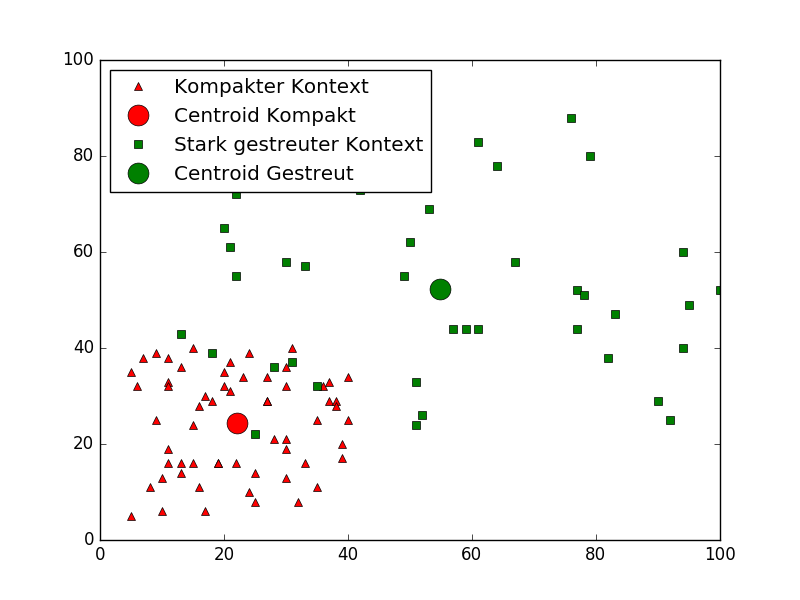
\includegraphics[width = \textwidth]{kontext}
    \caption{Streuung und Kompaktheit verschiedener Kontexte. Die beliebig dimensionalen Featurevektoren werden hier schematisch als Punkte im 2dimensionalen Raum dargestellt. Die Kontexte sind jeweils alle Featurevektoren des Kontextes eines Wortes.}
    \label{kontext}
\end{figure}

Ein geeignetes Maß für die Kompaktheit des Kontextes zu finden, ist also entscheidend. Hierbei lässt sich ausnutzen, dass die Menge an Featurevektoren, die über den Kontext eines Wortes festgelegt wird, die Form eines \emph{Clusters} annimmt. In der Literatur finden sich einige Ansätze zur Evaluierung von verschiedenen Clusteralgorithmen (Zitat Zitat Zitat). Für dieses Problem sind besonders Maße für die Kompaktheit eines einzelnen Clusters interessant, ohne dabei andere Cluster zu berücksichtigen. Ich möchte also für zwei zu vergleichende Wörter nicht wissen, wie gut ihre Kontexe in Cluster aufgeteilt wurden oder wie sehr die Cluster überlappen (obwohl das sicher auch einige interessante Informationen über die statistischen Eigenschaften der Kontexte liefern würde), sondern evaluieren, wie dicht oder kompakt die jeweiligen Cluster sind. Das Maß soll dann möglichst vom verwendeten Featureraum abstrahieren und die Kompaktheit von Clustern über verschiedenen Vektorräume miteinander vergleichbar machen.

Ein Konzept, das aus der Clusterevaluierung nutzbar gemacht werden kann, ist der \emph{Centroid} bzw. geometrische Schwerpunkt, der den Mittelpunkt aller Featurevektoren repräsentiert. Wie weit sind die einzelnen Featurevektoren vom Schwerpunkt entfernt? Hohe Distanz lässt auf eine weite Streuung schließen, niedrige Distanz auf Kompaktheit. Um das Maß nicht allzusehr zu verkomplizieren, habe ich zur Bestimmung der Verteilung der Distanz der einzelnen Featurevektoren zum Schwerpunkt den Durschnitt aller Distanzen gewählt.

Das Maß für die semantische Spezifität eines Begriffes berechnet sich also wie folgt:

\begin{defi}
Seien $X_i$ die Menge aller Featurevektoren derjenigen Wörter, mit denen das Wort $w_i$ in einer Kontextrelation steht (s.o.), und $c_i$ der geometrische Schwerpunkt von $X_i$. Dann ist der \textbf{Mean Distance to Centroid Score} $mdcs_i$

\begin{equation*}
   mdcs_i = \sum_{x_j \in X_i} \frac{ dist(x_j, c_i) }{|X_i|}
\end{equation*}
\end{defi}

\subsection{Getestete Maße}

\subsection{Wordpaare}

\subsection{Resultate}

\section{Ein Modell für Anglizismen}

\subsection{Textgrundlage}

\subsection{Verwendete Technologien}

\subsection{Resultate}

\section{Konklusion}

\section{Ausblick}

Word Sense Disambiuation!

Statistical Significance of Observed Difference

\nocite{han2011}
\nocite{heyer2008}
\nocite{manning1999}

\bibliography{spinfohausarbeit}

\end{document}